% Rebuild: pdflatex -output-directory=<build> mixed-conway-probe.tex
% SVG/PNG are direct page exports of that PDF (PyMuPDF get_svg_image/get_pixmap).
\documentclass[tikz,border=12pt]{standalone}
\usepackage[T1]{fontenc}
\usepackage{lmodern,amsmath,amssymb}
\usetikzlibrary{arrows.meta}
\definecolor{ink}{HTML}{183444}
\definecolor{blue}{HTML}{1B6780}
\definecolor{amber}{HTML}{AD601A}
\begin{document}
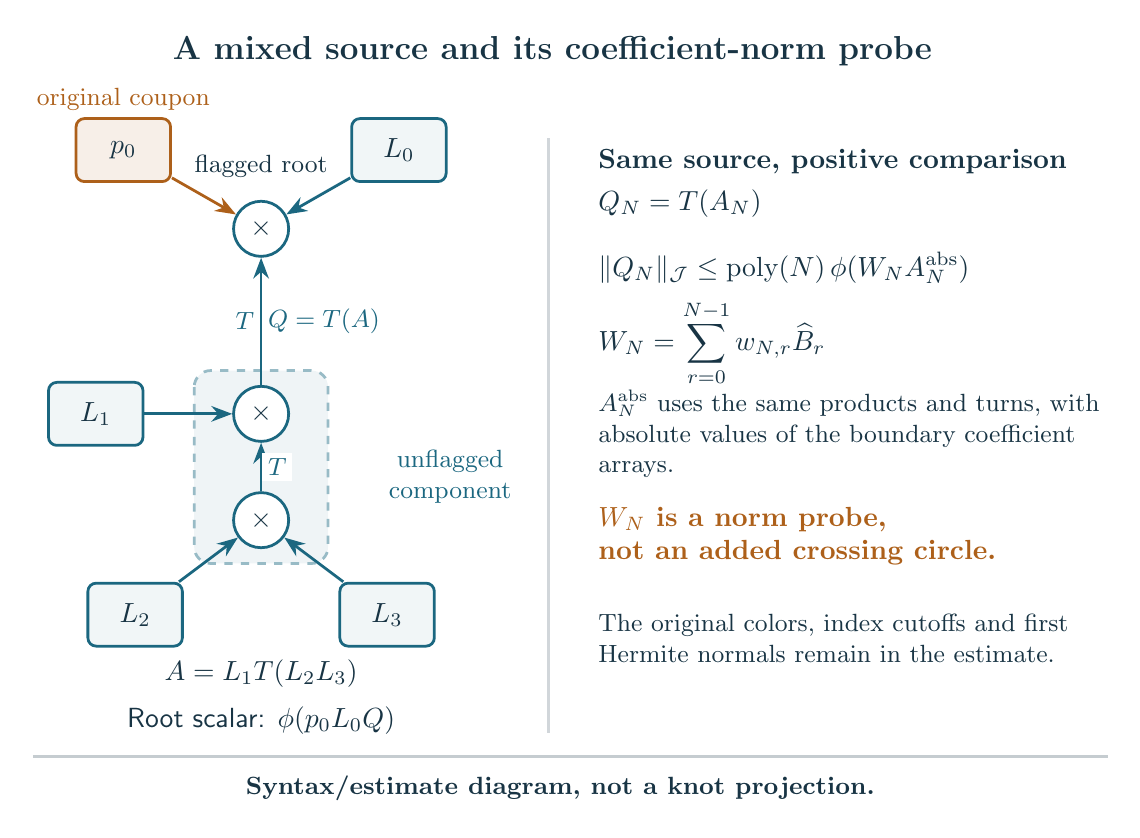
\begin{tikzpicture}[font=\sffamily,text=ink,line width=1pt,>=Stealth,
 hub/.style={circle,draw=blue,fill=white,minimum size=7mm,inner sep=1pt},
 module/.style={rounded corners=3pt,draw=blue,fill=blue!6,minimum width=12mm,minimum height=8mm},
 flag/.style={module,draw=amber,fill=amber!10},
 turn/.style={font=\small,fill=white,inner sep=2pt,text=blue}]
 \node[font=\large\bfseries] at (.2,4.9)
  {A mixed source and its coefficient-norm probe};
 \filldraw[fill=blue!7,draw=blue!45,dashed,rounded corners=6pt]
  (-4.35,.85) rectangle (-2.65,-1.6);
 \node[hub] (root) at (-3.5,2.65) {$\times$};
 \node[flag] (p0) at (-5.25,3.65) {$p_0$};
 \node[module] (L0) at (-1.75,3.65) {$L_0$};
 \node[font=\small,text=amber] at (-5.25,4.3) {original coupon};
 \node[font=\small] at (-3.5,3.45) {flagged root};
 \node[hub] (a) at (-3.5,.3) {$\times$};
 \node[hub] (b) at (-3.5,-1.05) {$\times$};
 \node[module] (L1) at (-5.6,.3) {$L_1$};
 \node[module] (L2) at (-5.1,-2.25) {$L_2$};
 \node[module] (L3) at (-1.9,-2.25) {$L_3$};
 \draw[amber,->] (p0)--(root);
 \draw[blue,->] (L0)--(root);
 \draw[blue,->] (a)--node[turn,left]{$T$}
                         node[turn,right]{$Q=T(A)$}(root);
 \draw[blue,->] (L1)--(a);
 \draw[blue,->] (b)--node[turn,right]{$T$}(a);
 \draw[blue,->] (L2)--(b);
 \draw[blue,->] (L3)--(b);
 \node[text=blue,font=\small,align=center] at (-1.1,-.5)
  {unflagged\\component};
 \node[align=center] at (-3.5,-3.3)
  {$A=L_1T(L_2L_3)$\\[5pt]
   Root scalar: $\phi(p_0L_0Q)$};
 \draw[ink!20] (.15,3.8)--(.15,-3.75);
 \node[anchor=west,font=\bfseries] at (.65,3.5)
  {Same source, positive comparison};
 \node[anchor=west,align=left] at (.65,2.55)
  {$\displaystyle Q_N=T(A_N)$\\[12pt]
   $\displaystyle \|Q_N\|_{\mathcal J}
       \le \operatorname{poly}(N)\,\phi(W_NA_N^{\rm abs})$};
 \node[anchor=west,align=left] at (.65,1.2)
  {$\displaystyle W_N=\sum_{r=0}^{N-1}w_{N,r}\widehat B_r$};
 \node[anchor=west,text width=6.4cm,align=left,font=\small] at (.65,.05)
  {$A_N^{\rm abs}$ uses the same products and turns,
   with absolute values of the boundary coefficient arrays.};
 \node[anchor=west,text width=6.4cm,align=left,text=amber,font=\bfseries] at (.65,-1.25)
  {$W_N$ is a norm probe,\\not an added crossing circle.};
 \node[anchor=west,text width=6.4cm,align=left,font=\small] at (.65,-2.55)
  {The original colors, index cutoffs and first Hermite normals remain in the estimate.};
 \draw[ink!25] (-6.4,-4.05)--(7.25,-4.05);
 \node[font=\small\bfseries,align=center] at (.3,-4.45)
  {Syntax/estimate diagram, not a knot projection.};
\end{tikzpicture}
\end{document}
